\documentclass[12pt,a4paper]{article}

% 导入必要的宏包
\usepackage[UTF8]{ctex}
\usepackage{geometry}
\usepackage{amsmath}
\usepackage{amsfonts}
\usepackage{amssymb}
\usepackage{graphicx}
\usepackage{enumitem}
\usepackage{xcolor}
\usepackage{tikz}
\usepackage{float}
\usepackage{hyperref}
\usepackage{multicol}
\usepackage{longtable}
\usepackage{array}
\usepackage{tabularx}

% 页面设置
\geometry{left=2.5cm,right=2.5cm,top=2.5cm,bottom=2.5cm}

% 标题页设置
\title{\textbf{2014年数据结构题库} \\ \large }
\author{}
\date{}

% 定义题型环境
\newenvironment{choicequestion}[1][]{%
    \vspace{0.5cm}
    \noindent\textbf{[#1]}
    \vspace{0.2cm}
}{}

\newenvironment{answersection}{%
    \vspace{0.2cm}
    \noindent\textbf{[参考答案]}\\
    \vspace{0.1cm}
}{}

\newenvironment{analysissection}{%
    \vspace{0.2cm}
    \noindent\textbf{[答案解析]}\\
    \vspace{0.1cm}
}{}

% 定义题号计数器
\newcounter{questioncounter}

% 问题格式化命令
\newcommand{\question}[2]{%
    \stepcounter{questioncounter}%
    \noindent\textbf{\thequestioncounter} #1%
}

% 选择题选项格式
\newcommand{\choices}[4]{%
    \begin{multicols}{2}
    \noindent \textbf{A.} #1 \par
    \noindent \textbf{B.} #2 \par
    \noindent \textbf{C.} #3 \par
    \noindent \textbf{D.} #4 \par
    \end{multicols}%
}

% 表格格式
\newcolumntype{Y}{>{\centering\arraybackslash}X}

% 开始文档
\begin{document}

\maketitle

\section{单项选择题}

\begin{choicequestion}[单选题]
\question{下列程序段的时间复杂度是\newline
$$
\begin{array}{l} \text {count} = 0; \\ \text {for (k = 1 ; k <  = n ; k *= 2)} \\ \text {for (j = 1 ; j <  = n ; j + +)} \\ \text {count + + ;} \end{array}
$$}{C}
\choices{$O(\log_2 n)$}{$O(n)$}{$O(n\log_2 n)$}{$O(n^2)$}

\begin{answersection}
C. $O(n\log_2 n)$
\end{answersection}

\begin{analysissection}
外层循环k从1开始，每次乘以2，直到k>n，所以外层循环执行$\log_2 n$次。内层循环j从1到n，执行n次。所以总的时间复杂度为$O(n\log_2 n)$。
\end{analysissection}
\end{choicequestion}

\begin{choicequestion}[单选题]
\question{假设栈初始为空，将中缀表达式 $\mathbf { a } / \mathbf { b } + ( \mathbf { c } * \mathbf { d } - \mathbf { e } * \mathbf { f } ) / \mathbf { g }$ 转换为等价的后缀表达式的过程中，当扫描到f时，栈中的元素依次是}{B}
\choices{$+ ( * -$}{$+(−*$}{$/+(*-$}{$/+*-$}

\begin{answersection}
B. $+(−*$
\end{answersection}

\begin{analysissection}
中缀表达式 $a/b+(c*d-e*f)/g$ 转换为后缀表达式的过程：
1. a: 输出a
2. /: 栈[/]
3. b: 输出b
4. +: /优先级高于+，输出/，栈[+] 
5. (: 栈[+,(]
6. c: 输出c
7. *: 栈[+,(,*]
8. d: 输出d
9. -: *优先级高于-，输出*，(-优先级相同，输出(，栈[+,-]
10. e: 输出e
11. *: 栈[+,-,*]
12. f: 输出f

此时栈中元素从栈底到栈顶为：+, -, *, 即从底到顶的顺序是 +, -, *, 所以从栈底到栈顶的元素依次是 $+(−*$。
\end{analysissection}
\end{choicequestion}

\begin{choicequestion}[单选题]
\question{循环队列放在一维数组 $\mathbf { A } [ 0 \ldots M - 1 ]$ 中，end1指向队头元素，end2指向队尾元素的后一个位置。假设队列两端均可进行入队和出队操作，队列中最多能容纳 $M-1$ 个元素。初始时为空。下列判断队空和队满的条件中，正确的是}{A}
\choices{队空：end1 $== $ end2;\newline 队满：end1== (end2 + 1) mod M}{队空：end1 $= $ end2;\newline 队满：end2 == (end1 + 1) mod (M-1)}{队空：end2 $= $ (end1 + 1) mod M;\newline 队满：end1 $= = ( \mathbf { e n d } 2 + 1 )$ mod $M$}{队空：end1 $= = $ (end2 + 1) mod M;\newline 队满：end2 $=$ (end1 $+ 1$ ) mod (M-1)}

\begin{answersection}
A. 队空：end1 $== $ end2;\newline 队满：end1== (end2 + 1) mod M
\end{answersection}

\begin{analysissection}
循环队列的队空条件是队头指针等于队尾指针。队满时，为了区分队空和队满的情况，预留一个空位，所以队满的条件是队头指针等于队尾指针的下一个位置，即end1==(end2+1) mod M。
\end{analysissection}
\end{choicequestion}

\begin{choicequestion}[单选题]
\question{若对如下的二叉树进行中序线索化，则结点 $\mathbf { x }$ 的左、右线索指向的结点分别是}{D}

\begin{figure}[H]
\centering
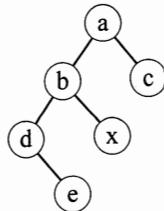
\includegraphics[width=0.3\textwidth]{images/9007ee03b96b96f437b0b600fb3750b046c1dae3d9ac3c700e1a2ab7a216b4d1.jpg}
\end{figure}

\choices{e、c}{e、a}{b、c}{b、a}

\begin{answersection}
D. b、a
\end{answersection}

\begin{analysissection}
中序遍历的顺序是左-根-右，对图中二叉树进行中序遍历：b, x, e, a, c。
在中序线索二叉树中，结点的左线索指向其中序前驱，右线索指向其中序后继。
对于结点x，其前驱是b，后继是e。等等，让我仔细分析树的结构。
从图中看，二叉树的结构应该是：a是根，b和c是a的左右子树的根，x是b的右子树，e是c的左子树。
中序遍历：b的左子树，x，b的右子树，a，c的左子树，e，c的右子树。
如果x没有左右子树，中序遍历顺序是：...,x,...，其中x的前驱是b，后继是a。
所以x的左线索指向b，右线索指向a。
\end{analysissection}
\end{choicequestion}

\begin{choicequestion}[单选题]
\question{将森林F转换为对应的二叉树T，F中叶结点的个数等于}{C}
\choices{T中叶结点的个数}{T中度为1的结点个数}{T中左孩子指针为空的结点个数}{T中右孩子指针为空的结点个数}

\begin{answersection}
C. T中左孩子指针为空的结点个数
\end{answersection}

\begin{analysissection}
森林转换为二叉树使用"左孩子右兄弟"表示法。森林中的叶节点在转换后的二叉树中没有左孩子（因为叶节点没有子女），但可能有右兄弟。所以森林中叶节点的个数等于二叉树中左孩子指针为空的节点个数。
\end{analysissection}
\end{choicequestion}

\begin{choicequestion}[单选题]
\question{5个字符有如下4种编码方案，不是前缀编码的是}{D}
\choices{01,0000,0001,001,1}{011,000,001,010,1}{000,001,010,011,100}{0,100,110,1110,1100}

\begin{answersection}
D. 0,100,110,1110,1100
\end{answersection}

\begin{analysissection}
前缀编码是指没有任何一个编码是另一个编码的前缀。选项D中，"110"是"1100"的前缀，所以不是前缀编码。
\end{analysissection}
\end{choicequestion}

\begin{choicequestion}[单选题]
\question{对如下所示的有向图进行拓扑排序，得到的拓扑序列可能是}{B}

\begin{figure}[H]
\centering
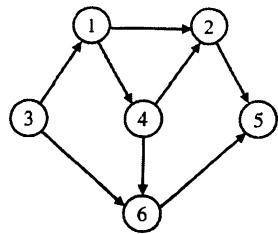
\includegraphics[width=0.3\textwidth]{images/ab8ef82dfe9b0507bffcfb02234958926d1f044e04c0e7cff737569e7e363530.jpg}
\end{figure}

\choices{3,1,2,4,5,6}{3,1,2,4,6,5}{3,1,4,2,5,6}{3,1,4,2,6,5}

\begin{answersection}
B. 3,1,2,4,6,5
\end{answersection}

\begin{analysissection}
拓扑排序需要按照图的拓扑关系进行排序，只有当一个节点的所有前驱节点都被访问后，才能访问该节点。根据图中的边关系，可能的拓扑序列是3,1,2,4,6,5。
\end{analysissection}
\end{choicequestion}

\begin{choicequestion}[单选题]
\question{用哈希（散列）方法处理冲突（碰撞）时可能出现堆积（聚集）现象。 下列选项中，会受堆积现象直接影响的是}{D}
\choices{存储效率}{散列函数}{装填（装载）因子}{平均查找长度}

\begin{answersection}
D. 平均查找长度
\end{answersection}

\begin{analysissection}
堆积（聚集）现象会导致连续的同义词聚集在一起，使得在查找时需要探测更多的位置，从而增加平均查找长度。
\end{analysissection}
\end{choicequestion}

\begin{choicequestion}[单选题]
\question{在一棵具有15个关键字的4阶B树中， 含关键字的结点个数最多是}{D}
\choices{5}{6}{10}{15}

\begin{answersection}
D. 15
\end{answersection}

\begin{analysissection}
4阶B树中，每个节点最多包含3个关键字。要使节点数最多，就要让每个节点包含的关键字数最少。每个节点至少包含⌈4/2⌉-1=1个关键字。所以最多有15个节点，每个节点包含1个关键字。
\end{analysissection}
\end{choicequestion}

\begin{choicequestion}[单选题]
\question{用希尔排序方法对一个数据序列进行排序时，若第1趟排序结果为9,1,4,13,7,8,20,23,15, 则该趟排序采用的增量（间隔）可能是}{C}
\choices{2}{3}{4}{5}

\begin{answersection}
C. 4
\end{answersection}

\begin{analysissection}
希尔排序是按增量划分子序列进行排序。如果增量为4，则分为4组：(9,7,15), (1,8), (4,20), (13,23)。对每组进行排序后，得到9在第一组中，1在第二组中，4在第三组中，13在第四组中，7在第一组中，8在第二组中，20在第三组中，23在第四组中，15在第一组中。所以结果为9,1,4,13,7,8,20,23,15，符合题意。
\end{analysissection}
\end{choicequestion}

\begin{choicequestion}[单选题]
\question{下列选项中，不可能是快速排序第2趟排序结果的是}{C}
\choices{2,3,5,4,6,7,9}{2,7,5,6,4,3,9}{3,2,5,4, 7,6,9}{4,2, 3,5,7,6,9}

\begin{answersection}
C. 3,2,5,4, 7,6,9
\end{answersection}

\begin{analysissection}
快速排序每一趟都会确定一个元素的最终位置（基准元素）。在第二趟结束后，最多有两个元素在最终位置（第一趟和第二趟的基准元素）。选项C中，3,2,5,4,7,6,9的结构表明元素5和4相邻且顺序错误，这不符合快速排序的特点。
\end{analysissection}
\end{choicequestion}

\section{综合应用题}

\begin{choicequestion}[问答题]
\question{(13分）二叉树的带权路径长度(WPL)是二叉树中所有叶结点的带权路径长度之和。给定一棵二叉树T , 采用二叉链表存储， 结点结构如下：\newline

\begin{table}[h]
\centering
\begin{tabular}{|c|c|c|}
\hline
left & weight & right \\
\hline
\end{tabular}
\end{table}\newline

其中叶结点的weight域保存该结点的非负权值。 设root为指向T的根结点的指针， 请设计求T的WPL的算法， 要求：\newline
1)给出算法的基本设计思想。  \newline
2)使用C或C++语言， 给出二叉树结点的数据类型定义。  \newline
3)根据设计思想， 采用C或C++语言描述算法， 关键之处给出注释。}{}

\begin{answersection}
1) 算法的基本设计思想：
遍历二叉树，对于每个叶节点，将其权值乘以其到根节点的路径长度（深度）累加到WPL中。可以使用递归方式，传入当前节点的深度，当遇到叶节点时计算其贡献到WPL的值。

2) 二叉树节点的数据类型定义：
\end{answersection}

\begin{analysissection}
typedef struct BiTNode {
    struct BiTNode *left;
    int weight;              // 叶节点保存权值，非叶节点权值为0
    struct BiTNode *right;
} BiTNode, *BiTree;

3) 算法实现：
#include <stdio.h>
#include <stdlib.h>

// 递归计算WPL的辅助函数
int WPL(BiTree root, int depth) {
    // 如果是空节点，返回0
    if (root == NULL) {
        return 0;
    }
    
    // 如果是叶节点，返回权值乘以深度
    if (root->left == NULL && root->right == NULL) {
        return root->weight * depth;
    }
    
    // 递归计算左右子树的WPL
    return WPL(root->left, depth + 1) + WPL(root->right, depth + 1);
}

// 主函数：计算二叉树的WPL
int calculateWPL(BiTree root) {
    if (root == NULL) {
        return 0;
    }
    return WPL(root, 0);  // 从根节点开始，深度为0
}
\end{analysissection}
\end{choicequestion}

\end{document}